\documentclass[a4paper,12pt]{article}

\usepackage[dutch]{babel}
\usepackage{fancyhdr}
\usepackage{graphicx}
\usepackage[pdftex,bookmarks=true]{hyperref}
\usepackage[utf8]{inputenc}
\usepackage{fullpage}
\usepackage{parskip}
\usepackage{float}
\usepackage{subcaption}
\usepackage{amsmath}
\usepackage{tikz}

\title{Samenvatting Probleem Oplossend Denken II \\ \large TIN 2 - HoGent}
\author{Lorenz Verschingel}

\begin{document}
\maketitle
\LARGE \textsc{Kansrekening}\normalsize
\section{Gebeurtenissen en hun kansen}
\subsection{Inleiding}
De kansrekening houdt zich bezig met de studie van gebeurtenissen of toevalsveranderlijken.

\subsection{Universum of uitkomstenruimte}
Het universum of de utkomstenruimte van een experiment is de verzameling van alle mogelijke uitkomsten van dit experiment en wordt genoteerd met $\Omega$.

Het is van belang dat de uitkomstenruimte volledig is: elke mogelijke
uitkomst van een experiment moet tot $\Omega$ behoren.
Bovendien moet elke uitkomst van een experiment overeenkomen met juist één element van $\Omega$.

\subsection{Gebeurtenis}
Een gebeurtenis is een deelverzameling van de uitkomstenruimte.
Een enkelvoudige of elementaire gebeurtenis is een \textit{singleton}.

Een \textit{samengestelde} gebeurtenis heeft cardinaliteit groter dan 1.

Gebeurtenissen die geen gemeenschappelijke uitkomsten hebben noemt men \textit{disjunct}.
Disjuncte gebeurtenissen kunnen dus nooit samen voorkomen.

\subsection{Kansen en kansruimte}
We wensen nu aan elke gebeurtenis A een getal te koppelen dat uitdrukt hoe waarschijnlijk het is dat deze gebeurtenis voorkomt bij het uitvoeren van een experiment.
We noemen dit getal de \textit{kans} of \textit{waarschijnlijkheid} van A, en we noteren deze kans als $P(A)$.

Het toekennen van kansen aan gebeurtenissen dient aan de volgende drie regels te voldoen:

\begin{enumerate}
\item Kansen zijn steeds positief: voor elke gebeurtenis $A$ geldt dat $P(A) \geq 0$.
\item De uitkomstenruimte heeft kans 1: $P(\Omega)=1$.
\item Wanneer $A$ en $B$ disjuncte gebeurtenissen zij dan is: $P(A\cup B)=P(A)+P(B)$.

Dit noemt men de \textbf{somregel}.
\end{enumerate}

Wanneer de functie $P$ aan de bovenstaande eigenschappen voldoet dan noemt ment het drietal $(\Omega, P(\Omega), P)$ een \textit{kansruimte}.

Kansen voldoen aan de volgende eigenschappen:
\begin{enumerate}
\item Voor elke gebeurtenis A geldt dat $P(\overline{A}) = 1-P(A)$

$1 = P(\Omega) = P(A\cup \overline{A}) = P(A) + P(\overline{A})$
\item De onmogelijke gebeurtenis heeft een kans nul: $P(\emptyset)=0$

$P(\emptyset)= P(\overline{\Omega}) = 1 - P(\Omega) = 0$
\item Als $A \subseteq B$ dan is $P(A)\leq P(B)$, dan geldt= $P(A) = P(B) - P(B\setminus A)$.
\item De \textbf{uitgebreide somregel} is: $P(A \cup B) = P(A) + P(B) - P(A \cap B)$

$P(A\cup B) = P(A \cup (B\setminus A))\\
= P(A) + P(B\setminus A)\\
= P(A) + P(B\setminus (A \cap B))\\
= P(A) +- P(B) - P(A \cap B)$
\end{enumerate}
\subsubsection{Eindig universum}
\textbf{Formule van Laplace}: $P(A)=\frac{\#(A)}{\#(\Omega)}$

De formule van Laplace is enkel van toepassing als alle kansen even waarschijnlijk zijn.

\subsection{Voorwaardelijke kansen en (on)afhankelijkheid van gebeurtenissen}
Als $P(B)>0$, dab is de \textbf{voorwaardelijke kans} dat $A$ voorkomt als gegeven is dat B voorkomt gedefinieerd is als:
$P(A|B)=\frac{P(A\cap B)}{P(B)}$

$P(A|B)$ spreken we uit als "De kans op A gegeven B".

Twee gebeurtenissen $A$ en $B$ zijn \textbf{onafhankelijk} als:
$P(A\cap B) = P(A)P(B)$

Bewijs: $P(A|B) = \frac{P(A\cap B)}{P(B)} =P(A) 
\Leftrightarrow P(A\cap B) = P(A)P(B)$

\subsubsection{De regel van Bayes}
$P(B_j|A) = 
\frac{P(B_j)P(P(A|B_j)}{\sum^n_{i=1}P(B_i)P(A|B_i)}$

Dit resultaat is belangrijk voor het opstellen van zogenaamde boomdiagrammen of beslissingsbomen in het kader van opeenvolgende beslissingen.

\section{Kans- of toevalsvariabelen}
\subsection{Inleiding}
Een \textit{kansvariabele} $X$ is een afbeelding van $\Omega$ naar $R$.
Deze afbeelding associeert met elke mogelijke uitkomst van een kansexperiment dus een reëel getal.

\subsection{Discrete kansvariabelen}
Een kansvariabele $X$ is \textit{discreet} wanneer $X$ slechts een eindig of aftelbaar oneindig aantal waarden aanneemt.
Dit wil zeggen dat: $bld(X)=\{x_1,x_2,\dots\}$.

$P(X=x_i)=P(\{\omega \cap \Omega |X(\omega)=x_i\})=f_X(x_i)$

\subsection{Continue kansvariabelen}
Een toevalsveranderlijke $X$ is \textit{continu} als er een functie $f_X$ van $R$ naar $R^+$ bestaat zodanig dat:
$F_X(x)=\int^x_{-\infty}f_X(y)dy$

De functie $f_X$ wordt de \textit{kansdichtheid} genoemd.

\subsection{Verwachtingswaarde en variantie}
\subsubsection{Discrete kansvariabele}
$E[x]= \sum_i^nx_iP(X=x_i)$

$E[x] = \mu$ = expected value = verwachtingswaarde = gemiddelde

$Var[x]=\sum_i^n(x_i-E[x])^2P(X=x_i)$

$Var[x] = \sigma^2$ = variantie = gemiddelde kwadratische afwijking

$\sigma$ = standaardafwijking

\subsubsection{Continue kansvariabele}
$E[x]=\int^\infty_{-\infty}xf_X(x)dx$

$Var[x]=\int^\infty_{-\infty}(x-\sigma_x)^2f_X(x)dx$

\subsubsection{Eigenschappen van verwachtingswaarde en variantie}
\begin{enumerate}
\item Als $X$ constant is, i.e. $X(\omega)=k$ voor alle elementen $\omega$ van  $\Omega$, dan is $E(X)=k$.
\item Als $a \in R$ een constante is, dan geldt:
$E(X+a)=E(X)+a)$

waaruit volgt dat: $E(X-\mu_X)=0$
\item Als $ a \in R$ een constante is, dan geldt:
$E(aX)=aE(X)$
\item Er geldt steeds dat:
$\sigma^2_X=E(X^2)-\mu^2_X$

Deze formule geeft de mogelijkheid om de variantie efficiënter te berekenen dan rechtstreeks via de definitie.
\item $\sigma^2_{X+a}=\sigma^2_X$
\item $\sigma^2_{aX}=a^2\sigma^2_X$
\end{enumerate}

\section{Kansverdelingen}
\subsection{Discrete kansverdelingen}
\subsubsection{De Bernoulliverdeling}
$x$ kan maar twee waarden aannemen.

\begin{table}[H]
\centering
\begin{tabular}{|c|c|c|}
\hline
x&0&1\\
\hline
$f_X(x)$ & 1-p & p\\
\hline
\end{tabular}
\end{table}
$\mu_X=0\times(1-p)+1\times p = p$

$\sigma^2_X=E[x^2]-E[x]^2=0^2\times (1-p)+1^2\times p - p^2 = p(1-p)=pq$

Het Bernouilliverdeling kan het best beschreven worden met het volgende voorbeeld:
één maal een muntstuk opgooien en kijken of je munt hebt.

\subsubsection{De binomiale verdeling}
$X\approx B(n,p)$

De binimiale verdeling kan het best beschreven worden met het volgende voorbeeld:
tien maal met een munt gooien en kijken hoeveel keer je munt hebt.

$f_X(k)=P(X=k)=C^k_np^kq^{n-k}=\binom{n}{k}p^kq^{n-k}$

met $\binom{n}{k}=\frac{n!}{k!(n-k)!}$

$\mu_X=np$

$\sigma^2_X=np(1-p)$

\subsubsection{De geometrische verdeling}
De geometrische verdeling kan het best beschreven worden met het volgende voorbeeld:
blijven gooien met een muntstuk tot je munt hebt.

$P(X=k) = (1-p)^{k-1}p$

$\mu_X = \frac{1}{1-q}$

$\sigma^2_X=\frac{q}{p^2}$

\textbf{De markov-eigenschap}

\begin{equation}
\begin{array}{rcl}
P(X>m+n|X>m)&=&\frac{P((X>m+n)\cap (X>n))}{P(X>n)}\\
&=& \frac{P(X>m+n)}{P(X>m)}\\
&=&\frac{q^{m+n}}{q^m}\\
&=&q^n\\
&=&P(X>n)
\end{array}
\end{equation}

\subsubsection{De Poisson verdeling}
De Poisson verdeling kan gezien worden als een binomiale verdeling met n  zeer groot en p $\approx$ 0.

$\Rightarrow np=\lambda$

$P(X=k)=e^{-\lambda}\frac{\lambda^k}{k!}$

$\mu_X = np=\lambda$

$\sigma^2_X=(np(1-p))=\lambda\times 1=\lambda$

\textbf{Het Poisson-proces}

$P(\text{k voorkomens in [0,t]})=e^{-\lambda t}\frac{(\lambda t)^k}{k!}$

\subsection{Continue kansverdelingen}
\subsubsection{Uniforme kansverdeling}
$\mu_X=\frac{a+b}{2}$

$\sigma^2_X=\frac{(b-a)^2}{12}$

\subsubsection{De exponentiële verdeling}
X $\rightarrow$ Poisson-proces met parameter $\lambda$.

T = tijd tot eerste voorkomen.

$P(T>t)=P(\text{0 voorkomens in[0,t]}) = e^{-\lambda t}\frac{(\lambda t)^k}{k!}=e^{-\lambda t}$

$\Rightarrow P(T\leq t) = 1-e^{-\lambda t}\text{ als t} \geq 0$

$\mu_T = \frac{1}{\lambda}$

$\sigma^2_T = \frac{1}{\lambda^2}$

De exponentiële verdeling voldoet aan de Markov-eigenschap: ze bezit geen geheugen.
\clearpage

\LARGE \textsc{Bomen en grafen}\normalsize
\section{Bomen}
\subsection{Terminologie}
Een \textit{gewortelde boom} T is een verzameling van \textit{toppen} die aan de volgende eigenschappen voldoet:

\begin{enumerate}
\item Er is één speciale top t die de \textit{wortel} van de boom wordt genoemd.
\item De andere toppen zijn verdeeld in $m\geq 0$ disjuncte verzameling T$_1$,\dots,T$_m$ die op hun beurt elk weer een gewortelde boom zijn.
\end{enumerate}

T$_1$,\dots,T$_m$ zijn \textit{deelbomen} van T.
De wortels t$_1$,\dots,t$_m$ van de deelbomen T$_1$,\dots,T$_m$ worden de \textit{kinderen} van de wortel t genoemd.
Omgekeerd is t de \textit{ouder} van t$_1$,\dots,t$_m$.
De toppen t$_1$,\dots,t$_m$ zijn \textit{broers} van elkaar.
De term \textit{afstammeling} en \textit{voorouder} zijn logische uitbreidingen van de kind/ouder terminologie.

Uit de recursieve definitie van een gewortelde boom volgt dat elke top in de boom uiteindelijk de wortel is van een deelboom die bevat is in de boom.
Het aantal deelbomen van een top wordt de \textit{graad} van die top genoemd.
Een \textit{blad} is een top met graad nul.
Een top die geen blad is wordt \textit{intern} genoemd.
De \textit{graad} van een boom wordt gedefinieerd als het maximum van de graden van zijn toppen.

\subsection{Datastructuren voor bomen}
\subsubsection{Array-van-kinderen voorstelling}
\begin{figure}[H]
	\centering
	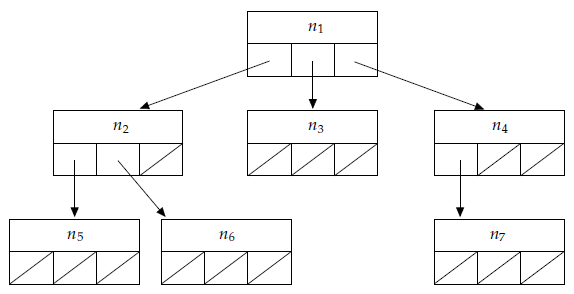
\includegraphics[width=.5\linewidth]{img/Array-van-kinderen}
  	\caption{Array-van-kinderen voorstelling}
  	\label{fig:Array-van-kinderen}
\end{figure}

De eenvoudigste manier om een boom voor te stellen is door rechtstreeks de vaderkind relatie te implementeren.
Dit betekent dat we een structuur Top definiëren die een veld heeft om de data van de top bij te houden, alsook een array van referenties
naar de kinderen van die top.
Wanneer een kind niet bestaat dan wordt dit voorgesteld door de referentie null.
De boom zelf bestaat uit een referentie naar zijn
wortel.

Aantal referenties: $n \times k$

Aantal gebruikte referenties: $n-1$

$\frac{\text{aantal gebruikte}}{\text{totaal}}
=\frac{n-1}{nk} 
\approx \frac{1}{k}$

\subsubsection{Eerste-kind-volgende-broer voorstelling}
\begin{figure}[H]
	\centering
	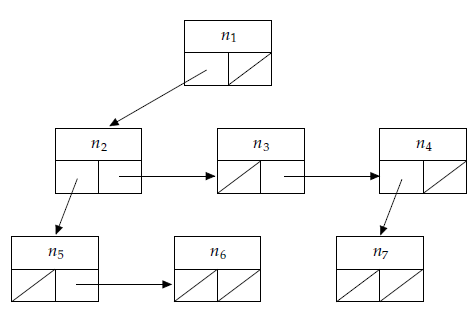
\includegraphics[width=.5\linewidth]{img/Eerste-kind-volgende-broer}
  	\caption{Eerste-kind-volgende-broer voorstelling}
  	\label{fig:Eerste-kind-volgende-broer}
\end{figure}

We kunnen een boom voorstellen op een manier die efficiënter met het geheugen omgaat.
In plaats van in elke top referenties naar al zijn kinderen op te slaan, houden we altijd juist twee referenties bij: een referentie naar zijn eerste kind, en een referentie naar zijn volgende broer.

Aantal referenties: $2n$

Aantal gebruikte referenties: $n-1$

$\frac{\text{aantal gebruikte}}{\text{totaal}}
=\frac{n-1}{2n} 
\approx \frac{1}{2}$

\subsection{Recursie op bomen}
\subsubsection{Alle toppen van een boom bezoeken}
Om een boom te doorlopen in preorde gaat men als volgt tewerk:
\begin{enumerate}
\item Bezoek de wortel van de boom.
\item Doorloop alle deelbomen van de wortel in preorde.
\end{enumerate}

Om een boom te doorlopen in postorde gaat men als volgt tewerk:
\begin{enumerate}
\item Doorloop alle deelbomen van de wortel in postorde.
\item Bezoek de wortel van de boom.
\end{enumerate}

Dit proces zal eindigen want wanneer de boom slechts uit één top bestaat.

\subsection{Binaire bomen}
\subsubsection{Definitie en eigenschappen}
Een \textit{binaire boom} is een verzameling toppen die
\begin{enumerate}
\item ofwel leeg is,
\item ofwel bestaat uit een wortel en twee disjuncte verzamelingen T$_l$ en T$_r$, die op hun beurt ook een binaire boom zijn.
We noemen T$_l$ en T$_r$ respectievelijk de linker- en rechterdeelboom van de wortel.
\end{enumerate}

\textbf{Eigenschappen}

In een binaire boom is het aantal toppen met diepte k hoogstens $2^k$.

Voor een (niet-lege) binaire boom T met een diepte $d\geq 0$ geldt dat:
$d+1\leq \#(T) \leq 2^{d+1}-1$

Bewijs:
\begin{equation}
\begin{array}{r c l}
\#(T) & = & \sum^d_{k=0}\text{aantal toppen met diepte k}\\
&\leq & \sum^d_{k=0}2^k\\
&=&1+2+4+\dots+2^k\\
&=&2^{d+1}-1\\
\end{array}
\end{equation}

\subsubsection{Voorstelling binaire boom}
\begin{figure}[H]
	\centering
	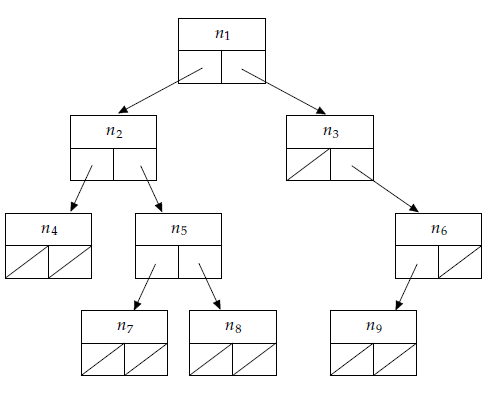
\includegraphics[width=.5\linewidth]{img/BinaireZoekboom}
  	\caption{Interne voorstelling van een binaire zoekboom}
  	\label{fig:InterneVoorstellingBinaireZoekboom}
\end{figure}
\subsubsection{Alle toppen van een binaire zoekboom bezoeken}
\textbf{Preorde}:

\begin{enumerate}
\item Bezoek de wortel van de boom.
\item Als de linkerdeelboom niet leeg is, doorloop de linkerdeelboom dan recursief in preorde.
\item Als de rechterdeelboom niet leeg is, doorloop de rechterdeelboom dan recursief in preorde.
\end{enumerate}

\textbf{Postorde}:

\begin{enumerate}
\item Als de linkerdeelboom niet leeg is, doorloop de linkerdeelboom dan recursief in postorde.
\item Als de rechterdeelboom niet leeg is, doorloop de rechterdeelboom dan recursief in postorde.
\item Bezoek de wortel van de boom.
\end{enumerate}

\textbf{Inorde}:

\begin{enumerate}
\item Als de linkerdeelboom niet leeg is, doorloop de linkerdeelboom dan recursief in inorde.
\item Bezoek de wortel van de boom.
\item Als de rechterdeelboom niet leeg is, doorloop de rechterdeelboom dan recursief in inorde.

\end{enumerate}

\subsection{Binaire zoekbomen}
Een \textit{binaire zoekboom} is een gelabelde binaire boom die aan een
bijzondere voorwaarde, de binaire zoekboomeigenschap, voldoet.

De \textit{binaire zoekboomeigenschap} is de volgende: voor elke top
x van de binaire zoekboom geldt dat alle toppen in de linkerdeelboom van x een label hebben dat kleiner is dan het label van x, terwijl voor alle toppen in de rechterdeelboom van x geldt dat hun label groter is dan het label van x.

\subsubsection{Opzoeken van een sleutel in een binaire zoekboom}
Om (recursief) te zoeken naar een bepaalde waarde x in een binaire zoekboom T volgt men de volgende stappen:

\begin{enumerate}
\item Wanneer de boom leeg is, geef dan ’niet gevonden’ terug.
\item Vergelijk x met de sleutel van de wortel.
	\begin{enumerate}
	\item Wanneer x kleiner is dan dit label, zoek dan (recursief) in de linkerdeelboom.
	\item Wanneer x groter is dan dit label, zoek dan (recursief) in de rechterdeelboom.
	\item Geef de wortel van de boom terug (x werd gevonden).
	\end{enumerate}
\end{enumerate}

\subsubsection{Toevoegen van een sleuten aan een binaire zoekboom}
We kunnen het toevoegen van een sleutel x aan een (niet-lege) binaire zoekboom als volgt recursief formuleren:
\begin{enumerate}
\item Vergelijk x met het label van de wortel.
	\begin{enumerate}
	\item Wanneer x kleiner is dan het label van de wortel, voeg dan x toe aan de linkerdeelboom wanneer die niet leeg is.
	Wanneer de linkerdeelboom leeg is vervang dan de (null)-referentie naar de linkerdeelboom door de referentie naar een nieuwe knoop met x als label.
	\item Wanneer x groter is dan het label van de wortel, voeg dan x toe aan de rechterdeelboom wanneer die niet leeg is.
	Wanneer de rechterdeelboom leeg is vervang dan de (null)-referentie naar de rechterdeelboom door de referentie naar een nieuwe knoop met x als label.
	\item Doe niets, want x behoort reeds tot de boom.
	\end{enumerate}
\end{enumerate}

\subsubsection{Verwijderen van een sleutel uit een binaire zoekboom}
Het verwijderen van een sleutel x start met het opzoeken van deze sleutel in de boom.
Er kunnen zich nu drie gevallen voordoen:
\begin{enumerate}
\item Sleutel is een blad:
	\begin{enumerate}
	\item Verwijder de referentie.
	\end{enumerate}
\item Sleutel is een top met één kind:
	\begin{enumerate}
	\item Referentie veranderen in ouder.
	\end{enumerate}
\item Sleutel is een top met 2 kinderen:
	\begin{enumerate}
	\item Zoek het minimum in de rechterboom.
	\item Vervang het te verwijderen element door de gevonden waarde.
	\item Verwijder het minimum in de rechterdeelboom.
	\end{enumerate}
\end{enumerate}

\subsubsection{Tijdscomplexiteit van de bewerkingen}
\begin{equation}
\begin{array}{r c l}
n & = & 2^{d+1}-1\\
& \approx & 2^{d+1}\\
&&\\
\multicolumn{3}{l}{\Rightarrow lg(n) \approx lg(2^{d-1})=d+1} 
\end{array}
\end{equation}

\subsection{Binaire hopen}
\subsubsection{Prioriteitswachtrij als binaire hoop}
Een \textit{complete binaire hoop} is een binaire boom van diepte d waarbij het aantal toppen met diepte $k < d$ maximaal (dus $2^k$) is.
De toppen met diepte d komen voor van "links naar rechts".

De \textit{ordeningseigenschap voor binaire hopen} zegt dat de
sleutel van elke top hoogstens gelijk is aan de sleutel van zijn kinderen.

\subsubsection{Implementatie van een binaire hoop}
\begin{figure}[H]
\centering
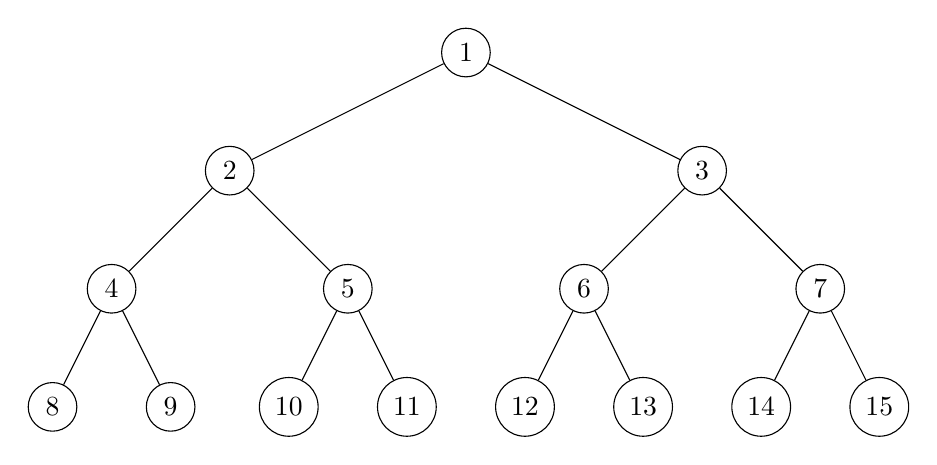
\begin{tikzpicture}
\node[circle,draw](z){1}
  child{
  	node[circle,draw]{2}
  		child{
  			node[circle,draw]{4}
  				child{
  					node[circle,draw]{8}
  				}
  				child{
  					node[circle,draw]{9}
  				}
  		}
  		child[missing]
  		child{
  			node[circle,draw]{5}
  			child{
  				node[circle,draw]{10}
  			}
  			child{
  				node[circle,draw]{11}
  			}
  		}
  }
  child[missing]
  child[missing]
  child[missing]
  child{
    node[circle,draw]{3} 
    	child{
    		node[circle,draw] {6}
    		child{
    			node[circle,draw]{12}
    		}
    		child{
    			node[circle,draw]{13}
    		}
    	}
    	child[missing]
    	child{
			node[circle,draw]{7}
			child{
    			node[circle,draw]{14}
    		}
    		child{
    			node[circle,draw]{15}
    		}  	
    	}
    };
\end{tikzpicture}
\caption{Voorstelling van een binaire hoop}
\label{fig:voorstellingBinaireHoop}
\end{figure}
De boom uit figuur~\ref{fig:voorstellingBinaireHoop} kan opgeslagen worden als een array.

Wanneer een top rangnummer i heeft, dan hebben zijn linker- en
rechterkind (als die bestaan) respectievelijk rangnummer $2i$ en $2i + 1$.

Omgekeerd geldt: wanneer een top rangnummer i heeft (en deze top is niet de wortel van de boom), dan heeft zijn ouder rangummer floor($i/2$).

\subsubsection{Opzoeken van het element met de kleinste sleutel}
Uit de ordeningseigenschap voor binaire hopen volgt dat het element met de kleinste sleutel steeds de wortel van de boom is.

\subsubsection{Toevoegen van een element}
\begin{enumerate}
\item Creëer een nieuw element.
\item Voeg dit element toe op de eerste beschikbare plaats.
Dit betekent dus als een nieuw blad, met rangnummer i, waarbij we er steeds voor zorgen dat het diepste niveau gevuld is van links naar rechts.
\item Op dit moment is het in het algemeen zo dat de ordeningseigenschap voor binaire bomen nu kan geschonden zijn tussen i en parent(i).
Indien dit zo is, verwissel dan i en parent(i). Dit herstelt de ordeningseigenschap tussen i en zijn ouder.
Eventueel is nu de ordeningseigenschap tussen parent(i) en parent(parent(i)) geschonden.
Indien dit zo is wissel dan beide elementen.
Ga zo verder tot de binaire hoop is hersteld.
\end{enumerate}

Dit proces wordt geïllustreerd in figuur~\ref{fig:ToevoegenBinaireHoop}.

\begin{figure}[H]
	\centering
	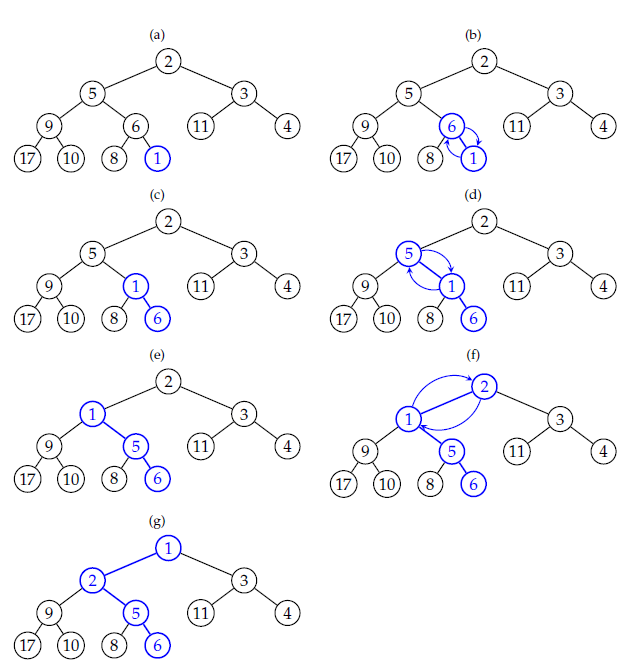
\includegraphics[width=.5\linewidth]{img/ToevoegenBinaireHoop}
  	\caption{Toevoegen van sleutel 1 aan een binaire hoop}
  	\label{fig:ToevoegenBinaireHoop}
\end{figure}

Het proces van het herstellen van de binaire hoop van beneden
naar boven, noemt men soms ook \textit{omhoog bubbelen}, omdat het nieuwe element
als het ware omhoog bubbelt in de hoop tot het op zijn correcte plaats staat.

\subsubsection{Verwijderen van het element met de kleinste sleutel}
\begin{enumerate}
\item Verwissel de wortel met het meest rechtse blad met de grootste diepte.
\item Verwijder het meest rechtse blad: de binaire hoop heeft nu een element minder.
\item Indien de ordeningseigenschap geschonden is in de wortel, herstel deze dan door de wortel en zijn kleinste kind i van plaats te verwisselen.
Indien de ordeningseigenschap nu geschonden is in i, herstel ze dan door i te verwisselen met de kleinste van zijn kinderen.
Ga zo verder tot de binaire hoop hersteld is.
\end{enumerate}

Dit proces wordt geïllustreerd in figuur~\ref{fig:VerwijderenBinaireHoop}.

\begin{figure}[H]
	\centering
	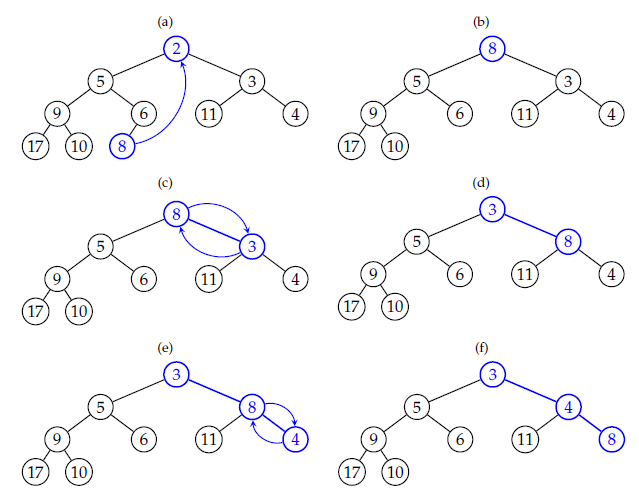
\includegraphics[width=.5\linewidth]{img/VerwijderenBinaireHoop}
  	\caption{Verwijderen van het kleinste element uit een binaire hoop}
  	\label{fig:VerwijderenBinaireHoop}
\end{figure}

Het proces dat gebruikt wordt bij het verwijderen van een element
noemt men soms ook \textit{omlaag bubbelen}, omdat het laatste element van de hoop omlaag bubbelt doorheen de hoop tot het op zijn juiste plaats staat.
\end{document}